\chapter{Image adjustment}

InVesalius cannot guarantee the correct image order; images may contain incorrect information, or do not follow the DICOM standard. Therefore, it is recommended to check if a lesion or an anatomical mark is on the correct side. If not, it is possible to use the flip image or swap axes tools. For image alignment, the rotation image tool can be used.

It is possible to mirror the image. To do so, select the \textbf{Tools} menu, click \textbf{Image}, then \textbf{Flip} and click on one of the following options (Figure~\ref{fig:menu_img_mirroring_axis_pt}):

\begin{itemize}
	\item Right - Left
	\item Anterior - Posterior
	\item Top - Botton
\end{itemize}

\begin{figure}[!htb]
\centering
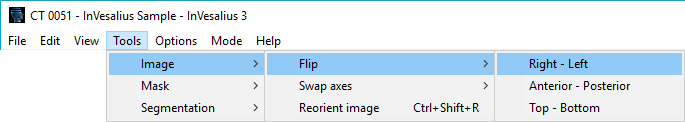
\includegraphics[scale=0.4]{../user_guide_figures/invesalius_screen/menu_img_mirroring_axis_en.png}
\caption{Menu to activate flip image tool.}
\label{fig:menu_img_mirroring_axis_pt}
\end{figure}


Figure~\ref{fig:mirrored} shows a comparison between the input image and the flipped image. All other orientations are also modified when the image is flipped.

\begin{figure}[!htb]
  \centering
  \subfloat[Input image]{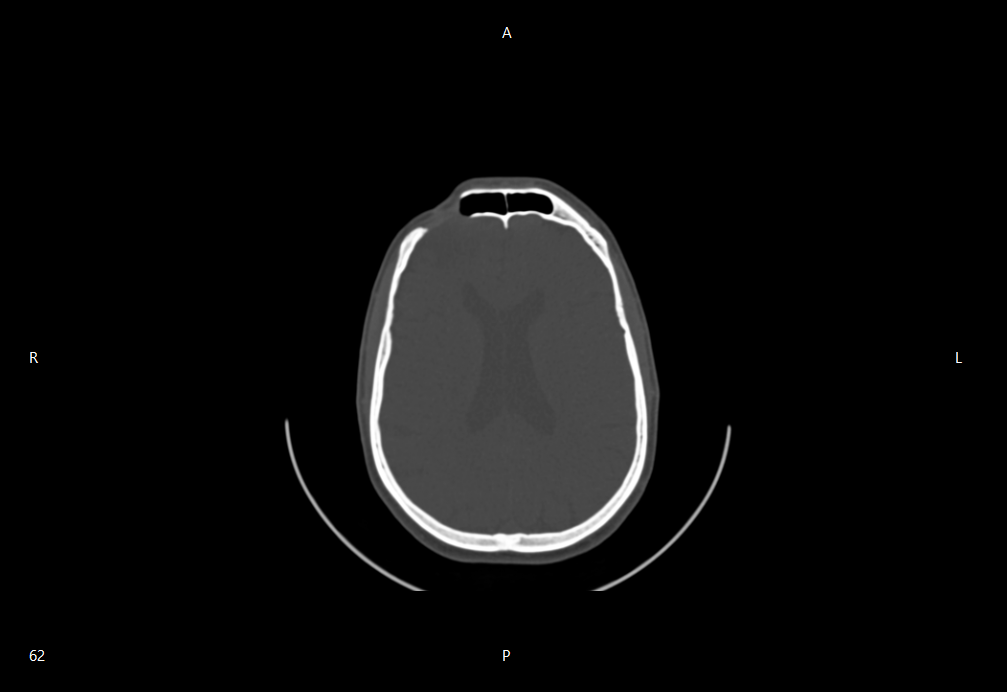
\includegraphics[width=0.45\textwidth]{../user_guide_figures/invesalius_screen/mirror_axial_en.png}}  \qquad
  \subfloat[Flipped image]{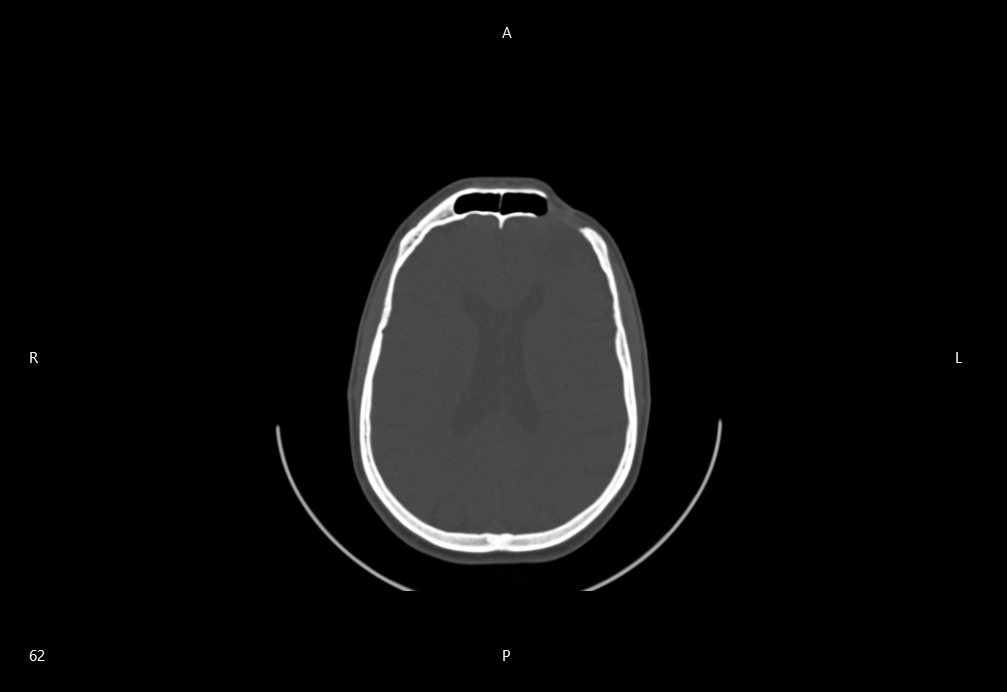
\includegraphics[width=0.45\textwidth]{../user_guide_figures/invesalius_screen/mirror_axial_mirrored_en.png}}
  \hfill
  \caption{Example of a right-left flipped image.}
  \label{fig:mirrored}
\end{figure}

\section{Swap axes}

The swap axes tool changes the image orientation, in the case that the image has been wrongly imported. To perform this, select the \textbf{Tools} menu, click \textbf{Image}, then \textbf{Swap Axes} and click on one of the following options (Figure~\ref{fig:menu_invert_axis}):

\begin{itemize}
	\item From Right-Left to Anterior-Posterior
	\item From Right-Left to Top-Bottom
	\item From Anterior-Posterior to Top-Bottom
\end{itemize}


The Figures~\ref{fig:invert_axis_axial} and~\ref{fig:invert_axis_axial_inverted}, shows an example of an image with inverted axes.

\begin{figure}[!htb]
\centering
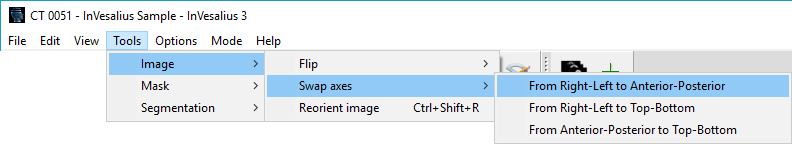
\includegraphics[scale=0.4]{../user_guide_figures/invesalius_screen/menu_invert_axis_en.png}
\caption{Menu to activate swap image tool.}
\label{fig:menu_invert_axis}
\end{figure}

\begin{figure}[!htb]
\centering
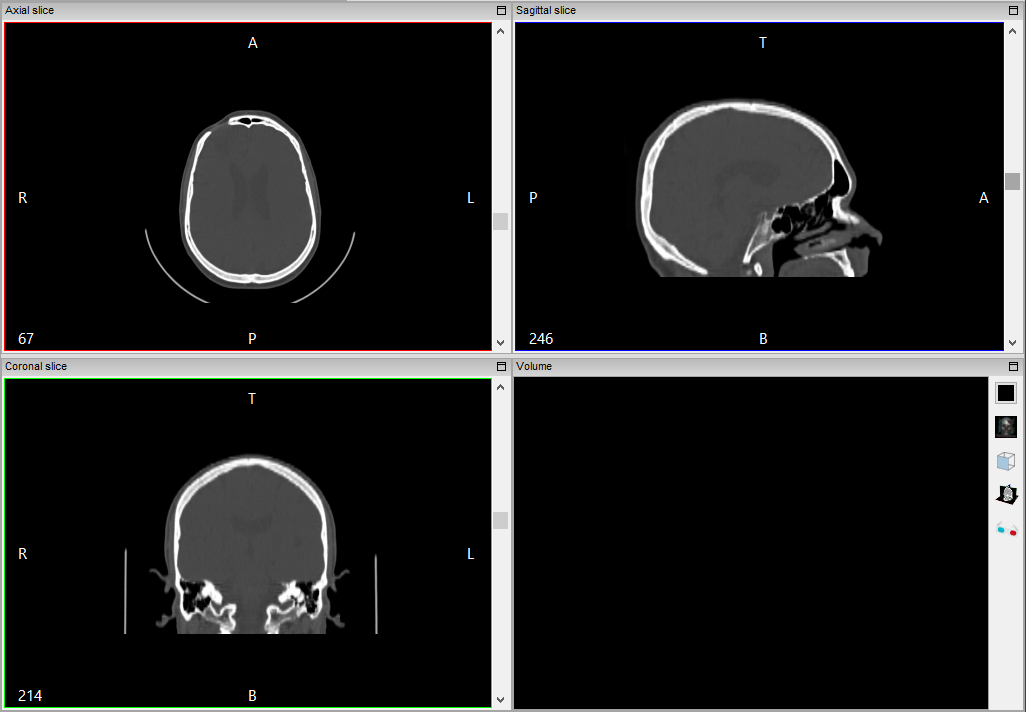
\includegraphics[scale=0.4]{../user_guide_figures/invesalius_screen/invert_axis_axial_en.png}
\caption{Images before swap axes - from Anterior-Posterior to Top-Bottom.}
\label{fig:invert_axis_axial}
\end{figure}

\begin{figure}[!htb]
\centering
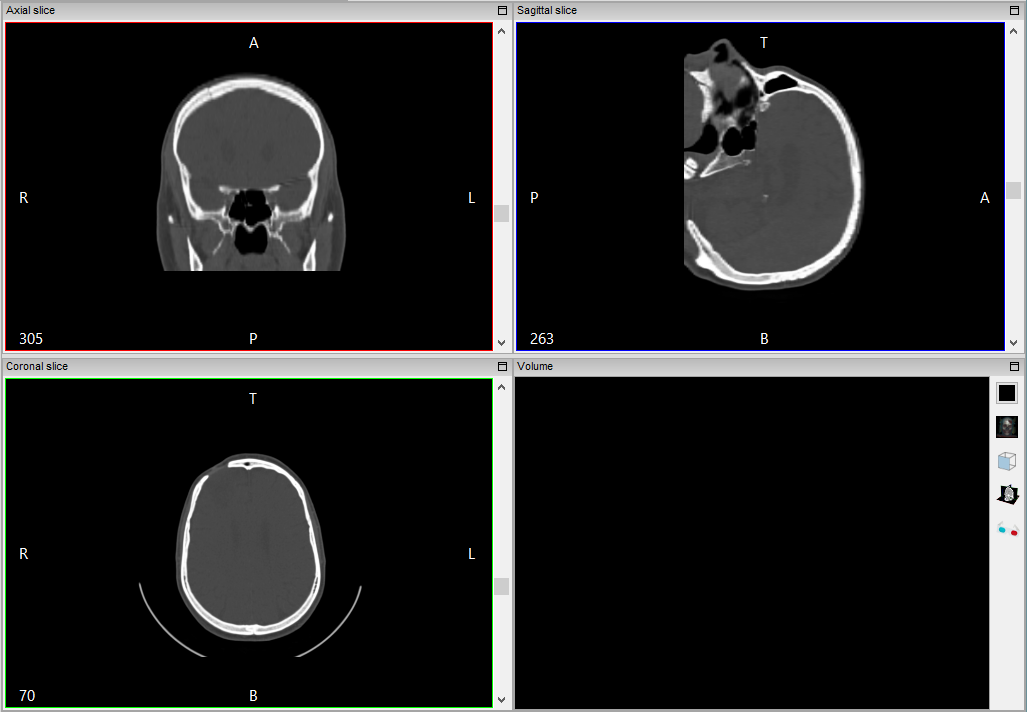
\includegraphics[scale=0.4]{../user_guide_figures/invesalius_screen/invert_axis_axial_inverted_en.png}
\caption{Images after swap axes - from Anterior-Posterior to Top-Bottom.}
\label{fig:invert_axis_axial_inverted}
\end{figure}

\section{Reorient image (Rotate)}

If it is necessary to align the image with a certain point of reference, e.g. anatomical marker, use the reorient image tool. To open this tool select the \textbf{Tools} menu, click \textbf{Image}, then \textbf{Reorient Image} (Figure~\ref{fig:menu_img_reorient}).

\begin{figure}[!htb]
\centering
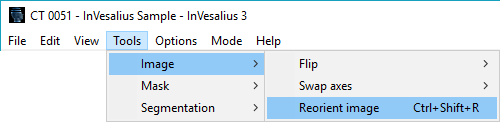
\includegraphics[scale=0.4]{../user_guide_figures/invesalius_screen/menu_img_reorient_en.png}
\caption{Menu to activate reorient image tool.}
\label{fig:menu_img_reorient}
\end{figure}

When this tool is activated a window is opened (Figure~\ref{fig:image_reorient_window}) showing orientation and by how many degrees the image was rotated.

\begin{figure}[!htb]
\centering
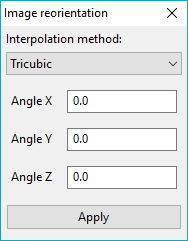
\includegraphics[scale=0.7]{../user_guide_figures/invesalius_screen/image_reorient_window_en.png}
\caption{Window that shows the reorientation image parameters.}
\label{fig:image_reorient_window}
\end{figure}

To start reorienting the image, define the interpolation method that will applied after rotation, by default is tricubic interpolation. The interpolation options are:

\begin{itemize}
	\item Nearest Neighbour
	\item Trilinear
	\item Tricubic
	\item Lanczos
\end{itemize}


Then, select the rotation point by keeping the \textbf{left} mouse button pressed between the two lines intersecting (Figure~\ref{fig:image_reorient_adjust_center}) at one orientation, e.g. axial, coronal or sagittal, and \textbf{drag} to the desired point.

\begin{figure}[!htb]
\centering
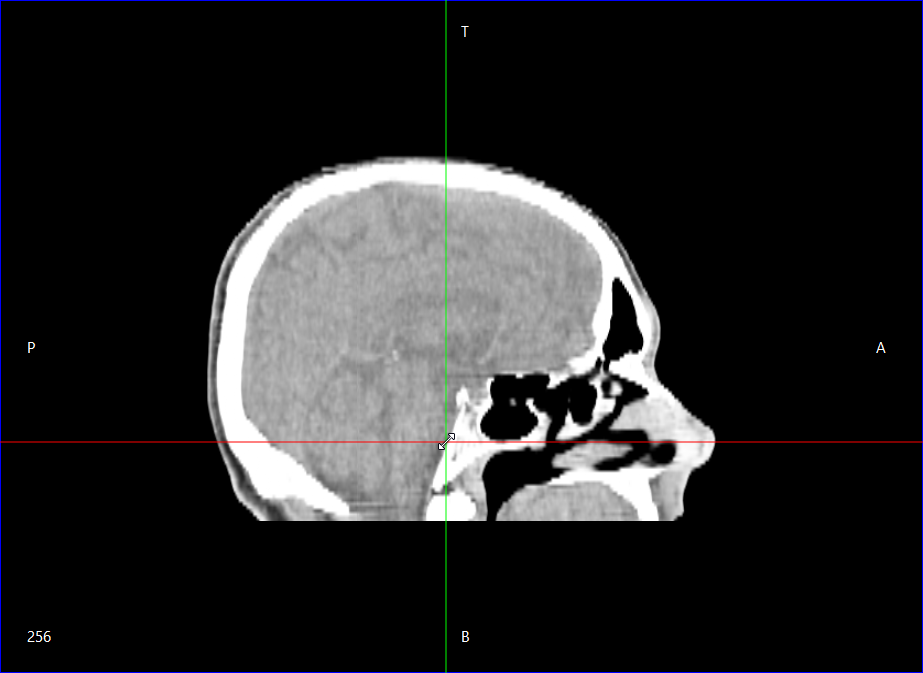
\includegraphics[scale=0.4]{../user_guide_figures/invesalius_screen/image_reorient_adjust_center_en.png}
\caption{Defining the axis of rotation of the image.}
\label{fig:image_reorient_adjust_center}
\end{figure}

To rotate the image it is necessary to keep the \textbf{left} mouse button pressed and \textbf{drag} until the reference point or anatomical marker stays aligned with one of the lines (Figure~\ref{fig:image_reorient_rotated}). After the image is in the desired position, click \textbf{Apply} in the parameter window (Figure~\ref{fig:image_reorient_window}). This may take a few moments depending on the image size. Figure~\ref{fig:image_reorient_rotated_applied} shows an image successfully reoriented.

\begin{figure}[!htb]
\centering
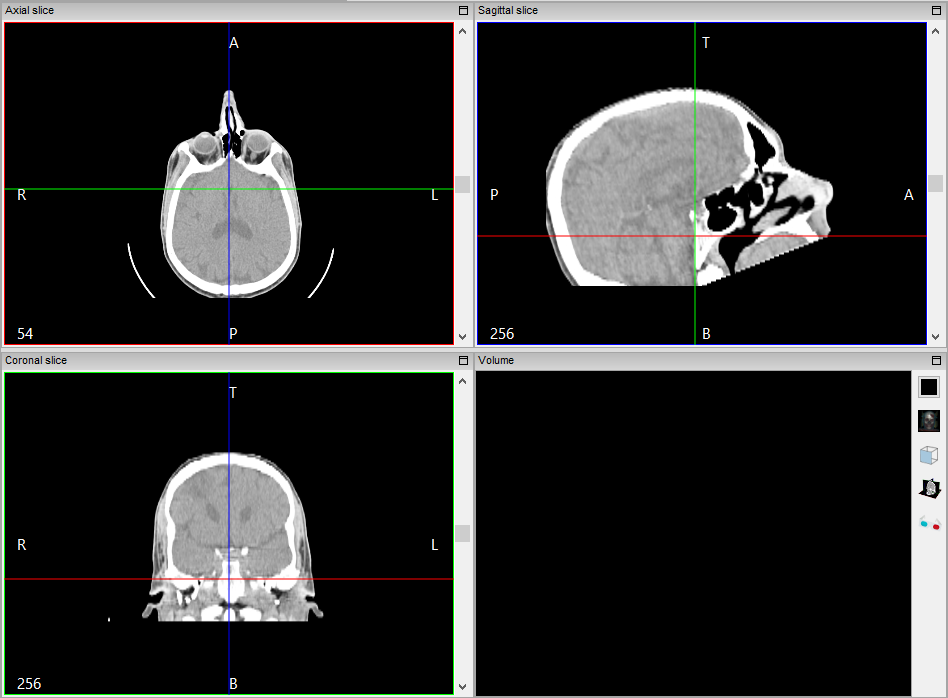
\includegraphics[scale=0.4]{../user_guide_figures/invesalius_screen/image_reorient_rotated_en.png}
\caption{Rotated image.}
\label{fig:image_reorient_rotated}
\end{figure}

\begin{figure}[!htb]
\centering
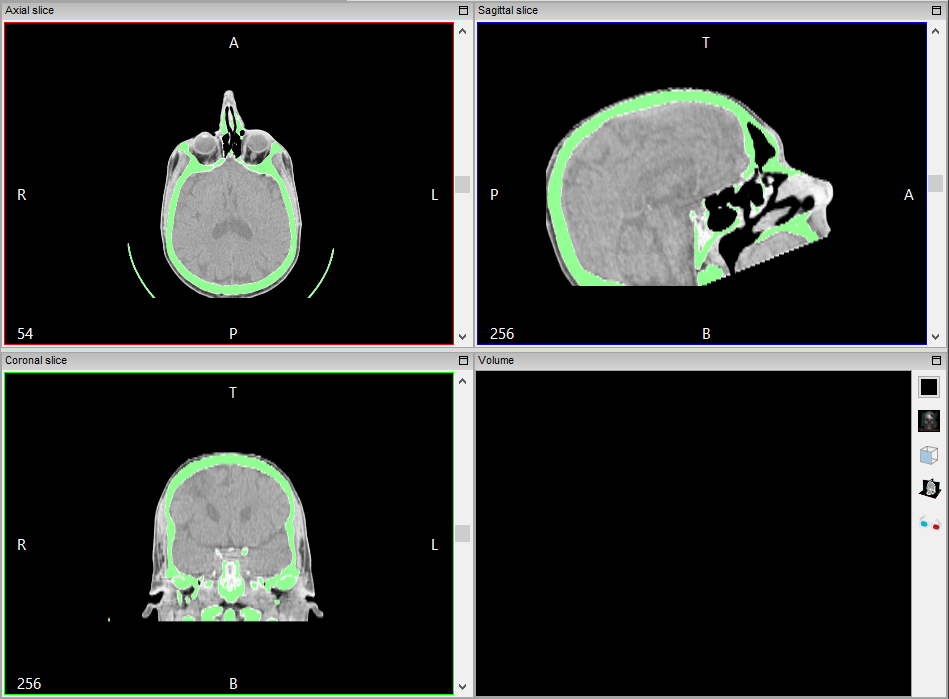
\includegraphics[scale=0.4]{../user_guide_figures/invesalius_screen/image_reorient_rotated_applied_en.png}
\caption{Rotated image after reorientation is done.}
\label{fig:image_reorient_rotated_applied}
\end{figure}
